\section{剪切自锁问题有限元无网格混合离散分析方法}
本章针对中厚板的剪切自锁问题,提出免剪切自锁的有限元无网格混合离散方案。首先,基于中厚板的本构特性,分析了传统有限元分析过程中产生剪切自锁现象的原因。基于LBB稳定系数误差估计和多项式空间,确定剪切自锁问题的最优约束比取值范围。随后,确定剪切自锁问题的有限元无网格混合离散方案,并通过典型弹性力学算例验证其正确性。
\section{中厚板问题}    
考虑如图\ref{ch_5:fig:mindlin_picture}所示中厚板,板厚为$h$,$\Omega$为板中面。在Mindlin假设下,中厚板考虑横向剪切变形,相应的控制方程由下式给出:
\begin{equation}\label{ch_5:eq:strong_mindlin}
    \begin{cases}
        M_{\alpha\beta,\beta} - Q_\alpha = 0 & \textrm{in}\; \Omega \\
        Q_{\alpha,\alpha} + \bar q = 0 & \textrm{in}\; \Omega \\    Q_\alpha n_\alpha = \bar Q & \textrm{on}\; \Gamma_Q \\
        M_{\alpha\beta} n_\beta = \bar M_\alpha & \textrm{on}\; \Gamma_M \\
        \varphi_\alpha = \bar \varphi_\alpha & \textrm{on}\; \Gamma_\varphi \\
        w = \bar w & \textrm{on}\; \Gamma_w \\
    \end{cases}
\end{equation}
式中希腊字母下标取为$1$或$2$,$M_{\alpha \beta}$ 可表示弯矩张量$ \boldsymbol{M}$ 的弯曲或扭转部分的分量,$Q_\alpha$为剪力张量$\boldsymbol{Q}$的分量,$\bar{q}$ 为垂直于板中面的分布荷载。
$\Gamma_w$和$\Gamma_\varphi$为挠度和转角的本质边界条件,$\bar{w}$和$\bar{\varphi}_\alpha$分别为本质边界条件上给定的挠度和转角。
$\Gamma_Q$ 和$\Gamma_M$ 为剪切力和弯矩的自然边界条件,$\bar Q$和$\bar{M}_{\alpha}$ 为自然边界上的等效剪力和法向弯矩。
$n_\alpha$为边界上外法向量$\pmb{n}$的分量。
\begin{figure}[!h]
    \centering 
        \includegraphics[scale=0.40]{ch_5/Mindlinplate.png}
        \caption{中厚板问题及边界条件示意图}\label{ch_5:fig:mindlin_picture}
\end{figure}
在平面应力假设下,对于各同向性线弹性材料,其本构关系表示为:
\begin{equation}\label{ch_5:eq:mindlin_M}
    M_{\alpha \beta}=-\frac{h^3}{12}C_{\alpha \beta \gamma\eta}\kappa_{\gamma\eta}=\frac{h^3}{12}C_{\alpha \beta \gamma\eta}\varphi_{\gamma,\eta}
\end{equation}
\begin{equation}\label{ch_5:eq:mindlin_Q}
    Q_{\alpha}= hkG\gamma_\beta =hkG(-\varphi_\beta+w_{,\beta})
\end{equation}
其中,$k$为剪切修正系数,通常取为$k=\frac{5}{6}$,
$G = \frac{E}{2(1+\nu)}$为剪切模量,
$\kappa_{\alpha\beta}$为曲率张量$\pmb\kappa$的分量,$\gamma_\alpha$为剪切应变张量$\pmb\gamma$的分量,它们的表达式为:
\begin{equation} \label{ch_5:eq:kappa}
    \kappa_{\alpha\beta}=-\varphi_{\alpha,\beta},\quad\gamma_\alpha=-\varphi_\alpha+w_{,\alpha}
\end{equation}
式中$C_{\alpha \beta \gamma\eta}$为在平面应力假设下四阶弹性张量的分量:
\begin{equation} 
    C_{\alpha \beta \gamma\eta}=\frac{E}{1-\nu^2}(\nu\delta_{\alpha\beta}\delta_{\gamma\eta}+\frac{1}{2}(1-\nu)(\delta_{\alpha\gamma}\delta_{\beta\eta}+\delta_{\alpha\eta}\delta_{\beta\gamma}))
\end{equation}

根据最小势能原理,强形式\eqref{ch_5:eq:strong_mindlin}所对应的势能泛函表达式为: 
\begin{multline}\label{ch_5:eq:potential_energy}
    \Pi(\boldsymbol{u}) =\int_{\Omega}\frac{1}{2}\kappa_{\alpha\beta}M_{\alpha\beta}d\Omega +\int_{\Omega}\frac{1}{2}\gamma_{\alpha}Q_{\alpha}d\Omega\\
    +\int_{\Gamma_{M}}\varphi_{\alpha}{\bar{M}_{\alpha}}d\Gamma-\int_{\Gamma_{Q}}{w}\bar {Q}d\Gamma-\int_{\Omega} w\bar{q}d\Omega
\end{multline}
其中,$\boldsymbol u = \{w, \varphi_1, \varphi_2\}^T$。对式\eqref{ch_5:eq:potential_energy}进行变分可得相对应的伽辽金弱形式:
\begin{equation}\label{ch_5:eq:weak_penalty_mindlin}
    \text{find}\; \boldsymbol u \in V, \quad
    a(\delta \boldsymbol u, \boldsymbol u) +
    a^s(\delta \boldsymbol u, \boldsymbol u) = 
    f(\delta \boldsymbol u)
    ,\quad \forall \delta \boldsymbol u \in V
\end{equation}
其中
\begin{align}
    a(\delta \boldsymbol u, \boldsymbol u) &= \int_{\Omega}\delta\kappa_{\alpha\beta}M_{\alpha\beta}d\Omega \\
    a^s(\delta \boldsymbol u, \boldsymbol u) &= \int_{\Omega}\delta\gamma_{\alpha}Q_{\alpha}d\Omega \\
    f(\delta \boldsymbol u) &= 
    -\int_{\Gamma_{M}}\delta\varphi_{\alpha}{\bar{M}_{\alpha}}d\Gamma+\int_{\Gamma_{Q}}{\delta{w}}\bar {Q}d\Gamma+\int_{\Omega} \delta{w}\bar{q}d\Omega
\end{align}

对于考虑横向剪切变形的中厚板,根据中厚板的本构关系\eqref{ch_5:eq:mindlin_M},\eqref{ch_5:eq:mindlin_Q},当其厚度减小$h\rightarrow 0$,$h \gg h^3$。在外力一定的情况下,弯矩本构方程中的材料系数远小于剪切力本构关系中的材料系数,导致剪切应变$\boldsymbol \gamma$远小于曲率$\boldsymbol \kappa$,即挠度和转角具有约束$w_{,\alpha} = \varphi_\alpha$。

在传统有限元法中,整个板中面$\Omega$由一组具有节点$\{\boldsymbol x_I\}_{I=1}^{n_u}$的构造网格离散,其中$n_u$是节点的数量。
挠度$w$及其变分$\delta w $,转角$\varphi_\alpha$及其变分$\delta \varphi_\alpha $可通过$x_I$处的节点系数和形函数进行近似:
\begin{equation}\label{ch_5:eq:w_h}
    w^h(\boldsymbol x) = \sum_{I=1}^{n_u} N_I(\boldsymbol x) w_I, \quad \delta w^h(\boldsymbol x) = \sum_{I=1}^{n_u} N_I(\boldsymbol x) \delta w_I
\end{equation}
\begin{equation}\label{ch_5:eq:varphi_h}
    \varphi^h_{\alpha}(\boldsymbol x) = \sum_{I=1}^{n_u} N_I(\boldsymbol x) \varphi_{\alpha I}, \quad \delta \varphi^h_{\alpha}(\boldsymbol x) = \sum_{I=1}^{n_u} N_I(\boldsymbol x) \delta \varphi_{\alpha I}
\end{equation}
其中,$N_I$为节点$x_I$处的形函数,$w_I$和$\varphi_{\alpha I}$节点系数张量。

结合式\eqref{ch_5:eq:kappa},\eqref{ch_5:eq:w_h}和\eqref{ch_5:eq:varphi_h},相应的近似曲率$\boldsymbol\kappa^h$和近似剪切应变$\boldsymbol\gamma^h$可表示为:
\begin{equation}
    \boldsymbol\kappa^h = 
    \begin{Bmatrix}
        \kappa^h_{11} \\ \kappa^h_{22} \\ 2\kappa^h_{12} 
    \end{Bmatrix} = -\sum_{I=1}^{n_u}
    \begin{bmatrix}
        0 & N_{I,1} & 0 \\ 0 & 0 & N_{I,2} \\ 0 & N_{I,2} & N_{I,1}
    \end{bmatrix}
    \begin{Bmatrix}
        w_I \\ \varphi_{1I} \\ \varphi_{2I}
    \end{Bmatrix} = - \sum_{I=1}^{n_u} \boldsymbol B^b_I \boldsymbol d_I
\end{equation}
\begin{equation}
    \boldsymbol\gamma^h = 
    \begin{Bmatrix}
        \gamma^h_1 \\ \gamma^h_2
    \end{Bmatrix} = \sum_{I=1}^{n_u}
    \begin{bmatrix}
        N_{I,1} & N_I & 0 \\
        N_{I,2} & 0 & N_I
    \end{bmatrix}
    \begin{Bmatrix}
        w_I \\ \varphi_{1I} \\ \varphi_{2I}
    \end{Bmatrix} = \sum_{I=1}^{n_u} \boldsymbol B^s_I \boldsymbol d_I
\end{equation}

将近似曲率和剪切应变代入到弱形式\eqref{ch_5:eq:weak_penalty_mindlin}可得下列里兹--伽辽金问题:
\begin{equation}\label{ch_5:eq:ritz_penalty_mindlin}
    \begin{split} 
        \text{Find}\,&(w^h,\boldsymbol{\varphi}^h_{\alpha})\in V_h\\
        &\int_{\Omega}\delta\kappa^h_{\alpha\beta}M_{\alpha\beta}d\Omega+\int_{\Omega}\delta\gamma^h_{\alpha}Q_{\alpha}d\Omega=\\
        &-\int_{\Gamma_{M}}\delta\varphi^h_{\alpha}{\bar{M}_{\alpha}}d\Gamma+\int_{\Gamma_{Q}}{\delta{w^h}}\bar {Q}d\Gamma+\int_{\Omega} \delta{w^h}\bar{q}d\Omega,\quad \forall(\delta w^h,\delta\varphi^h_{\alpha}) \in V_h
    \end{split}
\end{equation}
根据$\delta\boldsymbol\kappa^h$和$\delta\boldsymbol\gamma^h$的任意性,上述方程可简化为如下离散控制方程:
\begin{equation}\label{ch_5:eq:equilibrium_penalty}
    (\boldsymbol K^b + \boldsymbol K^s) \boldsymbol d = \boldsymbol f
\end{equation}
其中,$\boldsymbol K^b$为弯曲刚度矩阵,$\boldsymbol K^s$为剪切刚度矩阵,$\pmb{f}$为力向量,其分量具有以下形式:
\begin{equation}\label{ch_5:eq:stiffness_bending}
    \boldsymbol K^b_{IJ} = \frac{h^3}{12} \int_\Omega \boldsymbol B^{bT}_I \boldsymbol D \boldsymbol B^b_J d\Omega\\
\end{equation}
\begin{equation}\label{ch_5:eq:stiffness_shear}
    \boldsymbol K^s_{IJ} = h \int_\Omega \boldsymbol B^{sT}_I kG \boldsymbol B^s_J d\Omega
\end{equation}
\begin{equation}
    \boldsymbol f_I = \int_{\Gamma_Q} N_I \bar{\boldsymbol Q} d\Gamma - \int_{\Gamma_M} N_I \bar{\boldsymbol M} d\Gamma + \int_\Omega N_I \bar{\boldsymbol q} d\Omega
\end{equation}
式中,$\boldsymbol{D}$为平面应力弹性矩阵,等效剪力$\bar{\boldsymbol Q}$,法向弯矩$\bar{\boldsymbol M}$,分布荷载$\bar{\boldsymbol q}$的分量分别为:
\begin{equation}
    \bar{\boldsymbol Q} =  
    \begin{Bmatrix}
        \bar Q \\ 0 \\ 0
    \end{Bmatrix},
        \bar{\boldsymbol M} =
    \begin{Bmatrix}
        0 \\ \bar M_1 \\ \bar M_2
    \end{Bmatrix},
        \bar{\boldsymbol q} =
    \begin{Bmatrix}
        \bar q \\ 0 \\ 0
    \end{Bmatrix}
\end{equation}

\section{中厚板问题有限元无网格混合离散分析方法} 
从式\eqref{ch_5:eq:equilibrium_penalty},\eqref{ch_5:eq:stiffness_bending}和\eqref{ch_5:eq:stiffness_shear}可以看出,处理薄板问题时,当外力向量$\boldsymbol{f}$具有一定的数值时,厚度$h\rightarrow 0$剪切刚度矩阵$\boldsymbol{K^s}$和弯曲刚度矩阵所对应量纲的量级差将变大,从而导致大量纲项剪切刚度矩阵$\boldsymbol{K^s}$中的所有模态受到约束。用传统有限元法进行求解时,由于离散的有限元近似阶次较低,导致过多的弯曲自由度受到剪切约束的限制,挠度解将远小于实际情况,即出现剪切自锁现象。  

为建立中厚板问题的混合离散控制方程,在现有强形式的基础上引入了剪应力$\boldsymbol Q$和剪切应变$\boldsymbol \gamma$的关系式,此时强形式\eqref{ch_5:eq:strong_mindlin}可改写为:
\begin{equation}\label{ch_5:eq:strong_mindlin_mix}
    \begin{cases}
        M_{\alpha\beta,\beta} - Q_\alpha = 0 & \textrm{in}\; \Omega \\
        Q_{\alpha,\alpha} + \bar q = 0 & \textrm{in}\; \Omega \\
        \frac{Q_\alpha}{kGh} -\gamma_\alpha = 0 & \textrm{in}\; \Omega \\
        Q_\alpha n_\alpha = \bar Q & \textrm{on}\; \Gamma_Q \\
        M_{\alpha\beta} n_\beta = \bar M_\alpha & \textrm{on}\; \Gamma_M \\
        \varphi_\alpha = \bar \varphi_\alpha & \textrm{on}\; \Gamma_\varphi \\
        w = \bar w & \textrm{on}\; \Gamma_w \\
    \end{cases}
\end{equation}

引入剪切应力$\boldsymbol{Q}$作为拉格朗日乘子独立变量,可以得到拉格朗日乘子型剪切约束施加方案。此时能量泛函具有挠度$w$、转角$\boldsymbol{\varphi}$和剪切应力$\boldsymbol{Q}$三个变量:
\begin{multline}\label{ch_5:eq:potential_energy_mixed}
    \Pi(\boldsymbol{u},\boldsymbol Q) =\int_{\Omega}\frac{1}{2}\kappa_{\alpha\beta}M_{\alpha\beta}d\Omega +\int_{\Omega}\frac{1}{2}\gamma_{\alpha}Q_{\alpha}d\Omega
    + \int_\Omega \frac{1}{2} Q_\alpha (\gamma_\alpha - \frac{Q_\alpha}{kGh})d\Omega
    \\
    +\int_{\Gamma_{M}}\varphi_{\alpha}{\bar{M}_{\alpha}}d\Gamma-\int_{\Gamma_{Q}}{w}\bar {Q}d\Gamma-\int_{\Omega} w\bar{q}d\Omega
\end{multline}
对式\eqref{ch_5:eq:potential_energy_mixed}进行变分,并根据$\delta \boldsymbol u$和$\delta \boldsymbol Q$的任意性,可得利兹--伽辽金弱问题:
\begin{equation}\label{ch_5:eq:weak_mix}
    \text{find}\; \boldsymbol u \in V,\;\boldsymbol Q \in Q,\quad
    \left \{
    \begin{aligned}
        a(\delta \boldsymbol u, \boldsymbol u) + b(\delta \boldsymbol u,\boldsymbol Q) &= f(\delta \boldsymbol u) \quad &\forall \delta \boldsymbol u \in V \\
        b(\boldsymbol u, \delta \boldsymbol Q) +  c(\delta \boldsymbol Q,\boldsymbol Q)&= \boldsymbol 0 \quad &\forall \delta \boldsymbol Q \in Q
    \end{aligned}
    \right .
\end{equation}
其中
\begin{align}
    b(\delta \boldsymbol u, \boldsymbol Q) &= \int_{\Omega}\delta\gamma_{\alpha}Q_{\alpha}d\Omega \\
    c(\delta \boldsymbol Q, \boldsymbol Q) &= -\int_{\Omega}\frac{1}{kGh}\delta{Q}_{\alpha}{Q}_{\alpha}d\Omega
\end{align}

采用伽辽金法进行求解时,挠度$w$、转角$\boldsymbol{\varphi}$和剪切应力$\boldsymbol{Q}$可以采用不同的离散方式进行近似,形成混合离散框架。挠度$w$和转角$\boldsymbol{\varphi}$采用有限元形函数\eqref{ch_5:eq:w_h},\eqref{ch_5:eq:varphi_h}进行近似,剪切应力$\boldsymbol{Q}$通过再生核无网格形函数\eqref{ch_4:eq:mfshapefunction}进行近似,近似的剪切应力$\boldsymbol{Q}^h$及其变分可表示为:
\begin{equation}\label{ch_5:eq:Q_h}
    Q^h_\alpha(\boldsymbol x) = \sum_{K=1}^{n_q} \Psi_K(\boldsymbol x) \boldsymbol{q}_{K},\quad \delta Q^h_\alpha(\boldsymbol x) = \sum_{K=1}^{n_q} \Psi_K(\boldsymbol x) \delta \boldsymbol{q}_{ K}
\end{equation}
其中,$\boldsymbol{q}_{ K}$是节点系数,$\Psi_K$是对应的形函数。

根据$\delta\boldsymbol\kappa^h$、$\delta\boldsymbol\gamma^h$和$\delta\boldsymbol Q^h$的任意性,式\eqref{ch_5:eq:weak_mix}可简化为如下离散控制方程:
\begin{equation} \label{equilibrium_mindlin_mix}
    \begin{bmatrix}\boldsymbol{K}^{b}&\boldsymbol{K}^{sq}\\{\boldsymbol{K}^{sq}}^T&\boldsymbol{K}^{qq}\end{bmatrix}
    \begin{Bmatrix}\boldsymbol{d}\\\boldsymbol{q}\end{Bmatrix}=
    \begin{Bmatrix}\boldsymbol{f}\\\boldsymbol{0}\end{Bmatrix}
\end{equation}
式中,$\boldsymbol K^{sq}$为刚度矩阵中和挠度、剪切应力都有关的部分,$\boldsymbol K^{qq}$为刚度矩阵中只和剪切应力相关的部分,其分量分别为:
\begin{equation} 
    \boldsymbol K^{sq}_{IK} = \int_\Omega \boldsymbol B^{sT}_I \Psi_K d\Omega
\end{equation} 
\begin{equation} 
    \boldsymbol K^{qq}_{KL} = -\frac{1}{kGh} \int_\Omega \Psi_K \Psi_L \boldsymbol 1 d\Omega
\end{equation}

\section{剪切自锁问题最优体积约束比}

针对中厚板结构的剪切自锁问题,第\ref{LBB}章所提LBB稳定系数估计表达式\eqref{ch_3:eq:r23}、\eqref{ch_3:eq:r3}中,$\mathcal P$算子具有如下形式:
\begin{equation}\label{ch_5:eq:P}
    \mathcal P = \begin{bmatrix}
        \frac{\partial }{\partial x} & -1 & 0 \\
        \frac{\partial }{\partial y} & 0 & -1
    \end{bmatrix}
\end{equation}
同时,由式\eqref{ch_5:eq:w_h}、\eqref{ch_5:eq:varphi_h}和\eqref{ch_5:eq:Q_h}可知,位移节点上具有3个自由度而剪切力节点上具有2个自由度,相对应的约束比与最优约束比范围可定义为:
\begin{equation}
    r = \frac{3n_u}{2n_q}, \quad r_{opt} \ge \frac{3n_u}{2n_s} 
\end{equation}
其中,节点在求解域布置得当情况下,$n_p$与$n_s$可表示为:
\begin{align}
    2n_p &= \dim(V_{n_u} \setminus \ker \mathcal P_h \mathcal I_h) \\
    2n_s &= \dim(V_{n_u} \setminus \ker \mathcal P)
\end{align}

为确定$n_s$的大小,先对于维数为$n_u=3$的线性完备位移空间空间$V_3$进行分析。
此时多项式位移空间维度为$\dim V_3 = 9$,对多项式空间中的$\ker \mathcal P$单独列出整理,可得如下形式空间表达式:

\begin{equation}\label{ch_5:eq:base}
    V_3 = \mathrm{span} 
    \begin{Bmatrix}
        \underbrace{
        \begin{pmatrix} 1 \\ 0 \\ 0 \end{pmatrix},
        \begin{pmatrix} x \\ 1 \\ 0 \end{pmatrix},
        \begin{pmatrix} y \\ 0 \\ 1 \end{pmatrix}
        }_{\ker \mathcal P},
        \underbrace{
            \dots
        }_{V_3\setminus \ker \mathcal P}
    \end{Bmatrix}
\end{equation}
在这种情况下,$n_s=\frac{9-3}{2} = 3$。当$n_q\le n_s=3$时,$\beta_s>0$,即满足LBB稳定性条件。当$n_q>n_s=3$时$\beta_s=0$,不满足LBB稳定性条件。

进一步对$n_u=6$的二次完备多项式位移空间$V_6$采用同样的方式进行分析,整理后的空间可表示为:
\begin{equation}\label{ch_5:eq:base2}
    V_6 = \mathrm{span}
    \begin{Bmatrix}
        \underbrace{
        \begin{pmatrix} 1 \\ 0 \\ 0 \end{pmatrix},
        \begin{pmatrix} x \\ 1 \\ 0 \end{pmatrix},
        \begin{pmatrix} y \\ 0 \\ 1 \end{pmatrix},
        \begin{pmatrix} x^2 \\ 2x \\ 0 \end{pmatrix},
        \begin{pmatrix} xy \\ y \\ x \end{pmatrix},
        \begin{pmatrix} y^2 \\ 0 \\ 2y \end{pmatrix}
        }_{\ker \mathcal P}, 
        \underbrace{
            \dots
        }_{V_6\setminus \ker \mathcal P}
    \end{Bmatrix}
\end{equation}
此时,$\dim V_6 =18$,$n_s=\frac{18-6}{2}=6$。当$n_q\le n_s=6$时,$\beta_s>0$,即满足LBB稳定性条件。当$n_q>n_s=6$时,$\beta_s=0$,不满足LBB稳定性条件。按照上述的分析方式,可得表\ref{ch_5:tab:constraint}所示多项式阶数下$n_u$与$n_s$的关系。
\begin{table}[!h]
    \centering
    \caption{体积约束自由度}\label{ch_5:tab:constraint}
    \setlength{\tabcolsep}{10mm}
    \begin{tabular}{cccc}
        \toprule
            $\bar{n}_u$ & $3\bar{n}_u$ &$n$ &$ n_s$\\
        \midrule
        3  & 9  & 1 & 6 \\
        6  & 18 & 2 & 12 \\
        10 & 30 & 3 & 20 \\
        \vdots & \vdots & \vdots  & \vdots \\
        $\bar{n}_u$ & $3\bar{n}_u$ & $\lfloor\frac{\sqrt{1+8\bar{n}_u}-3}{2}\rfloor$ & $(n+1)(n+2)$ \\
        \bottomrule
    \end{tabular}
\end{table}

根据上述结果,满足LBB稳定性条件的最优约束比$r_{opt}$为:
\begin{equation}\label{ch_5:eq:best}
    r_{opt} \ge \frac{3n_u}{2n_s},\quad n_s = \frac{(n + 1)(n + 2)}{2},\quad n =\left \lfloor\frac{\sqrt{1+8n_u}-3}{2}\right \rfloor
\end{equation}

需要注意的是,上面提到的挠度自由度个数$3n_u$为施加本质边界条件之后的挠度自由度个数。根据文献{\citestyle{numbers}\cite{hughes2000}}中提出的约束比概念,由中厚板问题平衡微分方程\eqref{ch_5:eq:strong_mindlin_mix}中挠度、转角与剪切应力的控制方程数,可知传统剪切约束比为$3:2$,即$n_u:n_p=1:1$,从上式可知,传统剪切约束比无法满足LBB稳定性条件要求。

\subsection{剪切应力节点布置方案}

根据上述分析结果,为满足LBB稳定性条件,同时考虑编程实现的难易程度,本文针对剪切自锁问题的Tri3、Tri6、Quad4和Quad8位移单元提出了图\ref{ch_5:fig:mix_scheme}所示的剪切应力节点布置方案,该方案剪切应力节点同样在已有的位移节点中选取,以减小内存开销。
取去除掉可能受到强制边界条件约束的最外圈节点作为压力节点(二次单元多去除一圈),整体节点数满足所提LBB稳定系数估计式\eqref{ch_3:eq:r3}的要求。
在本章的数值算例中,mix--Tri3、mix--Tri6、mix--Quad4和mix--Quad8在不声明约束比的情况下,均采用这套离散方案。
\begin{figure}[H]
    \centering
        \begin{tabular}{c@{\hspace{24pt}}c}
            \includegraphics[width=0.25\textwidth]{ch_5/SquarePlate_tri3_8_msh.png} &
            \includegraphics[width=0.25\textwidth]{ch_5/SquarePlate_quad4_8_msh.png} \\
            mix--Tri3& mix--Quad4\\
            \includegraphics[width=0.25\textwidth]{ch_5/SquarePlate_tri6_8_msh.png} &
            \includegraphics[width=0.25\textwidth]{ch_5/SquarePlate_quad8_8_msh.png} \\
            mix--Tri6& mix--Quad8\\
            \raisebox{-0.3\height}{\includegraphics[width=14pt]{ch_5/legend_u.png}} :挠度节点 &
            \raisebox{-0.3\height}{\includegraphics[width=14pt]{ch_5/legend_q.png}} :剪切应力节点 
        \end{tabular}
        \caption{有限元无网格混合离散方案}\label{ch_5:fig:mix_scheme}
\end{figure}
\section{数值算例}

\subsection{固支方板问题}
如图\ref{ch_5:fig:plate}所示,一固支方板求解域为$\Omega=(0,1)\otimes(0,1)$,边长$L=1$,厚度为$h$,材料系数分别为杨氏模量$E=10.92\times10^6$、泊松比$\nu=0.3$板面内分布如图所示纵向非均布荷载:
\begin{equation} 
\begin{split} 
    \bar{q}(x,y) =&\frac{Eh^3}{12(1-\nu^2)}(12y(y-1)(5x^2-5x+1)(2y^2(y-1)^2+x(x-1)(5y^2-5y+\\
    &1))+12x(x-1)(5y^2-5y+1)(2x^2(x-1)^2+y(y-1)(5x^2-5x+1)))
\end{split} 
\end{equation}
该问题的精确解\cite{chinosi1995}为:
\begin{equation} 
    \begin{split} 
        w(x,y) =&\frac{1}{3}x^3(x-1)^3y^3(y-1)^3-\frac{2h^2}{5(1-\nu)}(y^3(y-1)^3x(x-1)(5x^2\\
        &-5x+1)+x^3(x-1)^3y(y-1)(5y^2-5y+1))\\
        \theta_1(x,y) =& y^3(y-1)^3x^2(x-1)^2(2x-1)\\
        \theta_2(x,y) =& x^3(x-1)^3y^2(y-1)^2(2y-1)
    \end{split}  
\end{equation}
\begin{figure}[H]
    \centering 
        \includegraphics[scale=0.7]{ch_5/plate.png}
        \caption{固支方板问题模型}\label{ch_5:fig:plate}
\end{figure}

如图\ref{ch_5:fig:plate_msh}所示,固支方板求解域采用均布的$8\times 8$、$16\times 16$、$32\times 32$和$64\times 64$有限元单元近似位移。对于采用线性和二次无网格近似的固支方板算例,其相对影响域大小分别取作1.5和2.5。

\begin{figure}[!ht]
    \centering
        \begin{tabular}{c@{\hspace{24pt}}c}
            \includegraphics[width=0.29\textwidth]{ch_5/SquarePlate_8_msh.png} &
            \includegraphics[width=0.29\textwidth]{ch_5/SquarePlate_16_msh.png} \\
            $8\times 8$ & $16\times 16$ \\
            \includegraphics[width=0.29\textwidth]{ch_5/SquarePlate_32_msh.png} &
            \includegraphics[width=0.29\textwidth]{ch_5/SquarePlate_64_msh.png} \\
            $32\times 32$ & $64\times 64$ \\
        \end{tabular}
        \caption{固支方板问题节点离散}\label{ch_5:fig:plate_msh}
\end{figure}

首先对有限元Tri3和Tri6单元在不同约束比下的位移和应力误差进行了分析。图\ref{ch_5:fig:plate_l2}为分析的结果,蓝色和绿色折线为Tri3单元和Tri6单元在位移节点数$n_u$固定的情况下,位移和应力误差随剪切应力节点数$n_q$变化的折线图。误差值越往下,表示结果越精确。图中竖直虚线表示上述LBB稳定系数估计下得到的最优约束比阙值,虚线左边满足LBB稳定性条件,右边则不满足。从图中可以看出,位移误差在最优约束比阙值附近始终保持在一定的数值,而当剪切应力节点在最优约束比范围内,应力误差逐渐减小。当剪切应力节点逐步增加,并超过最优约束比范围后,应力误差快速增大。结果与上述LBB稳定系数测试结果一致。

为验证上一节所提出的离散方案,对Tri3、Tri6、Quad4和Quad8单元在传统最优约束比($r=3:2$)和所提混合离散方案($r=r_{opt}$)下的误差进行对比。图\ref{ch_5:fig:SquarePlate_u}为固支方板问题的位移误差和应力误差对比图,从图中可以看出,对于位移误差但Tri6单元传统最优约束比($r=3:2$)下的位移误差无法达到理论误差收敛率,而混合离散方案($r=r_{opt}$)均可达到理论误差收敛率。;对于应力误差,混合离散方案($r=r_{opt}$)的计算精度优于传统最优约束比($r=3:2$),并且Tri6单元传统最优约束比($r=3:2$)下的压力误差无法达到理论误差收敛率,不满足LBB稳定性条件,而混合离散方案($r=r_{opt}$)均可达到理论误差收敛率。图\ref{ch_5:fig:plate_tri_q}和图\ref{ch_5:fig:plate_quad_q}为固支方板问题的压力云图。从图中可以看出传统最优约束比($r=3:2$)下的应力云图出现了明显的压力振荡现象,而混合离散方案($r=r_{opt}$)完全没有压力振荡现象。
\clearpage
\begin{figure}[H]
    \centering
    \begin{subcaptiongroup}[htbp]
        \begin{tabular}{c@{\hspace{0pt}}c}
        $\log_{10}\Vert \boldsymbol u - \boldsymbol u_h \Vert_V$ & $\log_{10}\Vert p - p_h \Vert_Q$\\
          \raisebox{-0.7\height}{\includegraphics[width=0.42\textwidth]{ch_5/u_nu81.png}}
        & \raisebox{-0.7\height}{\includegraphics[width=0.42\textwidth]{ch_5/q_nu81.png}}\\
          \raisebox{-0.7\height}{\includegraphics[width=0.42\textwidth]{ch_5/u_nu289.png}}
        & \raisebox{-0.7\height}{\includegraphics[width=0.42\textwidth]{ch_5/q_nu289.png}}\\
        \raisebox{-0.7\height}{\includegraphics[width=0.42\textwidth]{ch_5/u_nu1089.png}}
        & \raisebox{-0.7\height}{\includegraphics[width=0.42\textwidth]{ch_5/q_nu1089.png}}\\
        \raisebox{-0.7\height}{\includegraphics[width=0.42\textwidth]{ch_5/u_nu4225.png}}
        & \raisebox{-0.7\height}{\includegraphics[width=0.42\textwidth]{ch_5/q_nu4225.png}}\\
        \end{tabular}
    \end{subcaptiongroup}
    \caption{固支方板问题误差与剪切应力节点数的关系}\label{ch_5:fig:plate_l2}
\end{figure}
\begin{figure}[!h]
    \centering
    \begin{subcaptiongroup}
        \begin{tabular}{c@{\hspace{5pt}}c}
          \raisebox{-0.8\height}{\includegraphics[width=0.36\textwidth]{ch_5/u_tri.png}}
        & \raisebox{-0.8\height}{\includegraphics[width=0.36\textwidth]{ch_5/q_tri.png}}\\
        \raisebox{-0.8\height}{\includegraphics[width=0.36\textwidth]{ch_5/u_quad.png}}
        & \raisebox{-0.8\height}{\includegraphics[width=0.36\textwidth]{ch_5/q_quad.png}}\\
        \end{tabular}
    \end{subcaptiongroup}
    \caption{固支方板问题误差对比}\label{ch_5:fig:SquarePlate_u}
\end{figure}

\begin{figure}[!h]
    \centering
    \begin{subcaptiongroup}
        \begin{tabular}{c@{\hspace{0pt}}c}
         \raisebox{-0.7\height}{\includegraphics[width=0.35\textwidth]{ch_5/SquarePlate_mix_tri3_q1_32_32.png}}
         & \raisebox{-0.7\height}{\includegraphics[width=0.35\textwidth]{ch_5/SquarePlate_mix_tri3_q11_64_64.png}}\\
         mix-Tri3($r=3:2$)&mix-Tri3($r=r_{opt}$)\\
         \raisebox{-0.7\height}{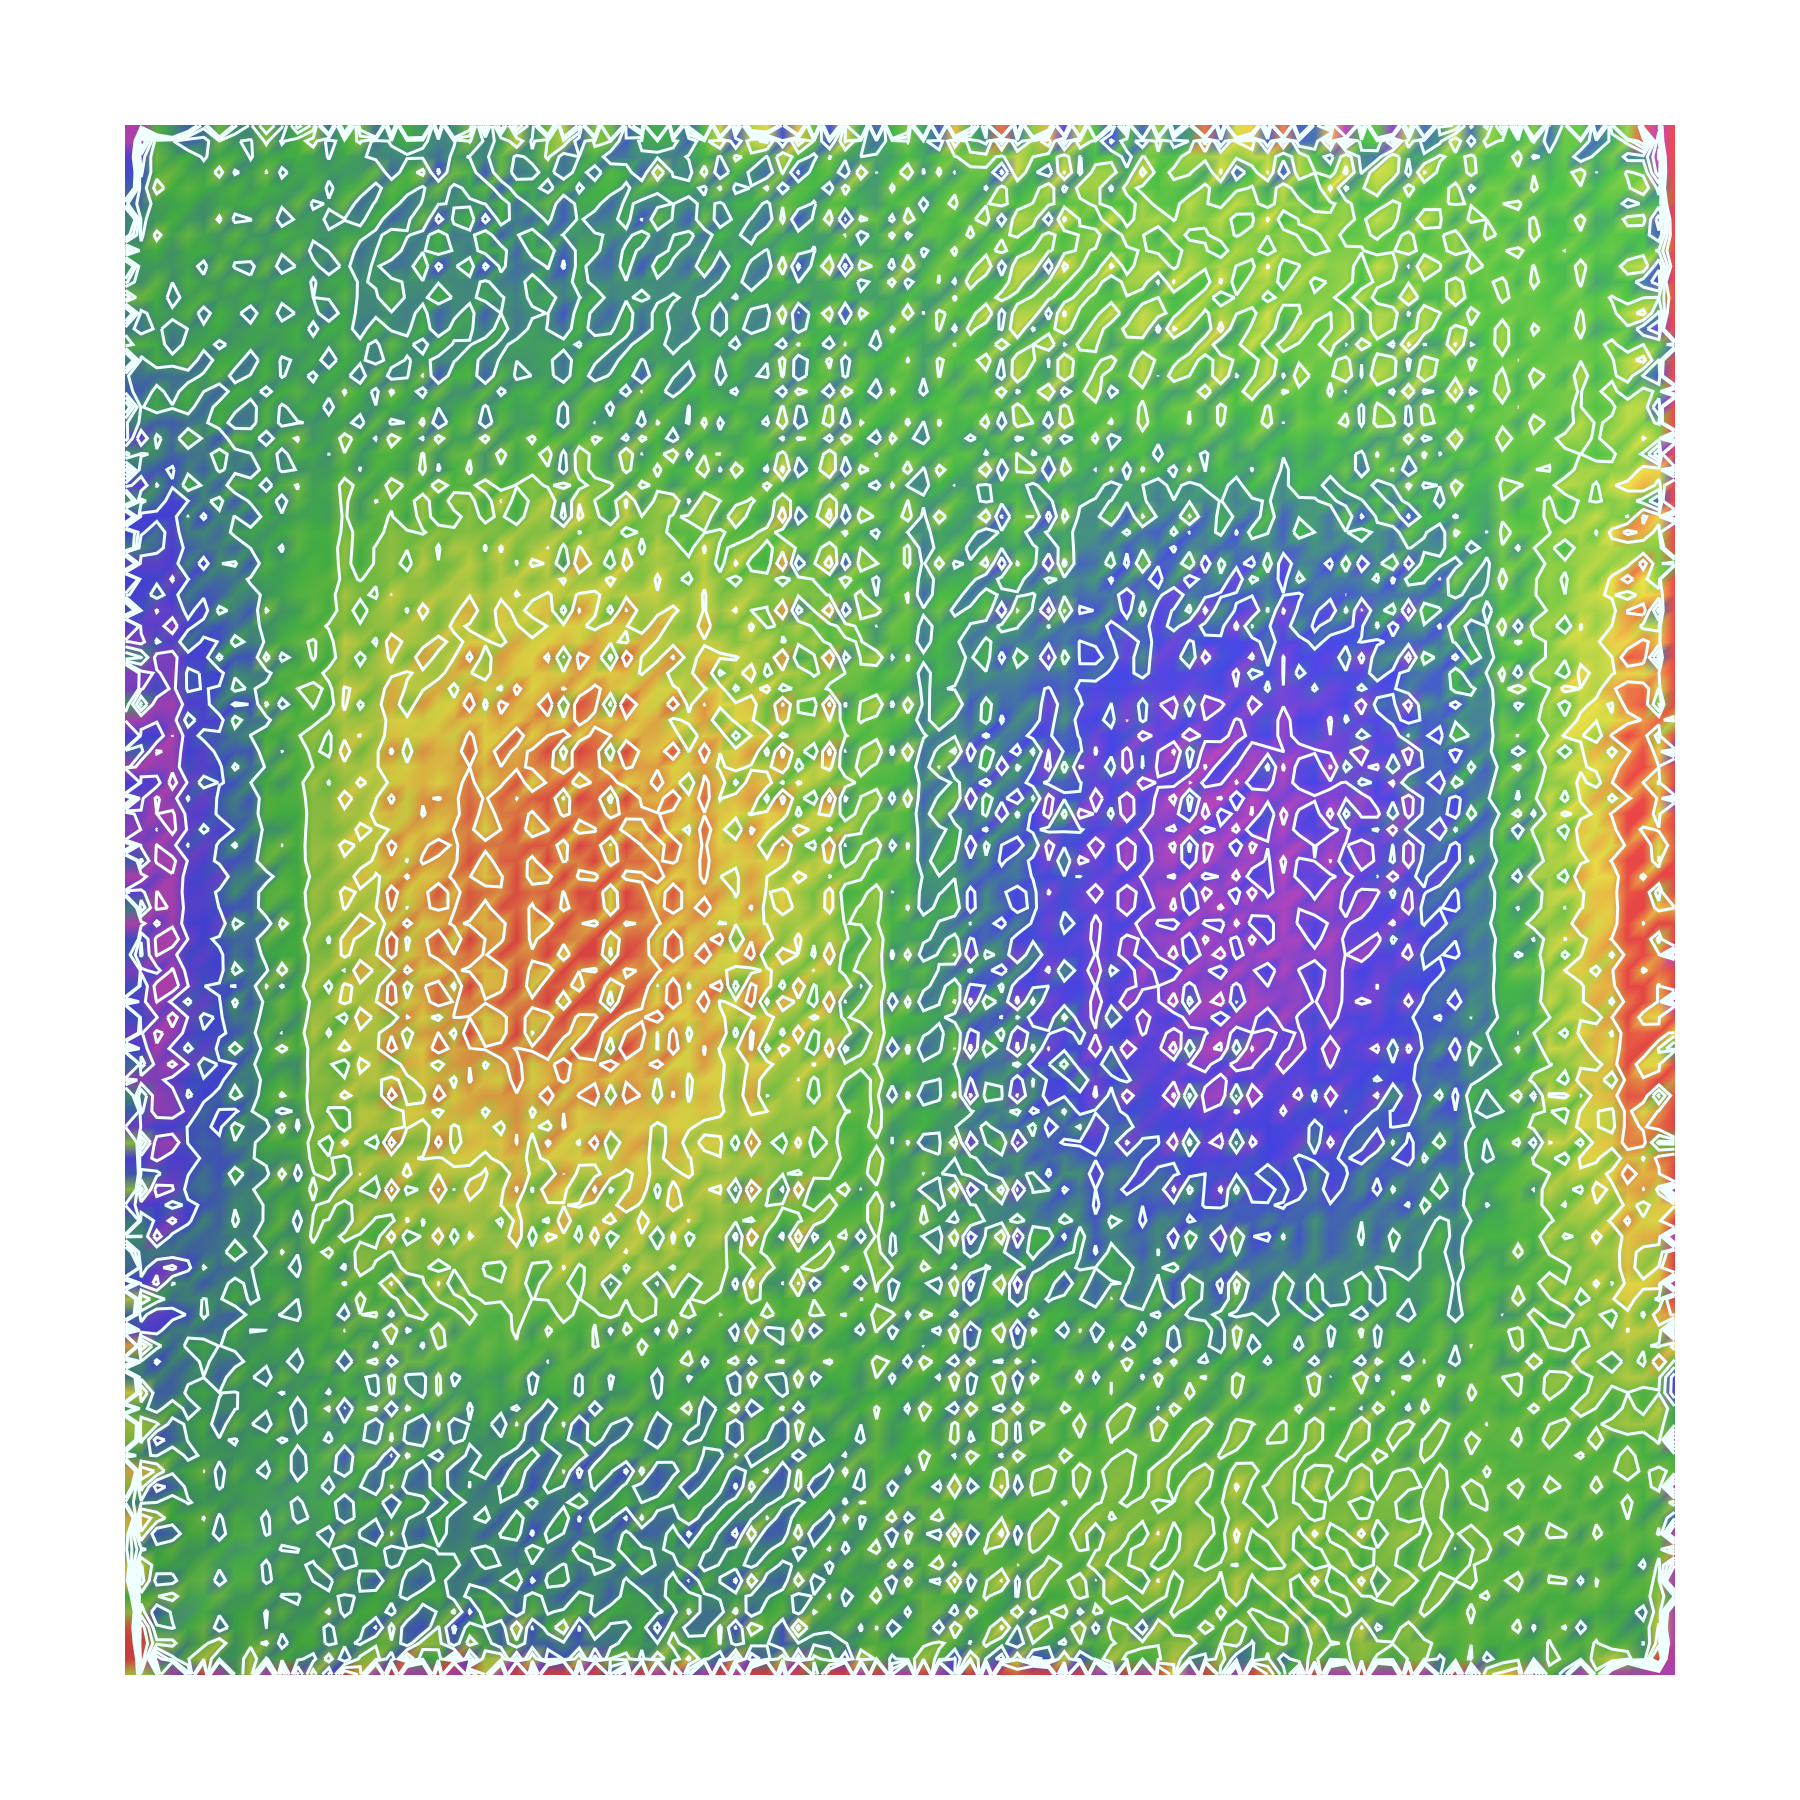
\includegraphics[width=0.35\textwidth]{ch_5/SquarePlate_mix_tri6_q1_32_32.png}}
        & \raisebox{-0.7\height}{\includegraphics[width=0.35\textwidth]{ch_5/SquarePlate_mix_tri6_q11_32_32.png}} \\
        mix-Tri6($r=3:2$)&mix-Tri6($r=r_{opt}$) \\
        \end{tabular}
    \end{subcaptiongroup}
    \caption{固支方板问题三角形单元应力云图}\label{ch_5:fig:plate_tri_q}
\end{figure}


\begin{figure}[!h]
    \centering
    \begin{subcaptiongroup}
        \begin{tabular}{c@{\hspace{0pt}}c}
            \raisebox{-0.7\height}{\includegraphics[width=0.35\textwidth]{ch_5/SquarePlate_mix_quad4_q1_32_32.png}}
            & \raisebox{-0.7\height}{\includegraphics[width=0.35\textwidth]{ch_5/SquarePlate_mix_quad4_q11_64_64.png}}\\
            mix-Quad4($r=3:2$)&mix-Quad4($r=r_{opt}$)\\
            \raisebox{-0.7\height}{\includegraphics[width=0.35\textwidth]{ch_5/SquarePlate_mix_quad8_q1_32_32.png}}
           & \raisebox{-0.7\height}{\includegraphics[width=0.35\textwidth]{ch_5/SquarePlate_mix_quad8_q11_32_32.png}} \\
           mix-Quad8($r=3:2$)&mix-Quad8($r=r_{opt}$) \\
        \end{tabular}
    \end{subcaptiongroup}
    \caption{固支方板问题四边形单元应力云图}\label{ch_5:fig:plate_quad_q}
\end{figure}

\subsection{Razzaque斜板问题}
考虑如图\ref{ch_5:fig:Razzaque_plate}所示斜板问题,其中斜板的边长为$L=100$,厚度为$h$,板内作用竖直向下的均布荷载作用$\bar{q}=1$,材料系数分别为杨氏模量$E=1085$、泊松比$\nu=0.31$。该斜板中心A点位移$\bar w_A$的参考解\cite{Katili1993}为:
\begin{equation} 
    \bar{w_A}=w_c\times10^2\frac{D}{\bar{q}L^4}
\end{equation}
\begin{figure}[H]
    \centering 
        \includegraphics[scale=0.6]{ch_5/xie plate.png}
        \caption{Razzaque斜板问题模型}\label{ch_5:fig:Razzaque_plate}
\end{figure}

Razzaque斜板问题求解域采用如图\ref{ch_5:fig:Razzaque_msh}所示的有限单元近似位移。此时,Tri3和Quad4单元位移节点数$n_u$为1089,Tri6单元位$n_u$为4225,Quad8单元$n_u$为3201。对于采用线性和二次无网格近似的Razzaque斜板问题,其相对影响域大小分别取1.5和2.5。

\begin{figure}[!h]
    \centering 
        \includegraphics[scale=0.4]{ch_5/MorleysAcuteSkewPlate_tri3_32_msh.png}
        \caption{Razzaque斜板问题节点离散}\label{ch_5:fig:Razzaque_msh}
\end{figure}

图\ref{ch_4:fig:Cook_membrane_p}为Razzaque斜板问题的Tri3、Tri6、Quad4和Quad8单元传统最优约束比($r=3:2$)和所提混合离散方案($r=r_{opt}$)的压力云图。
\begin{figure}[H]
    \centering
    \begin{subcaptiongroup}
        \begin{tabular}{c@{\hspace{0pt}}c@{\hspace{0pt}}c@{\hspace{0pt}}c}
     \raisebox{-0.7\height}{\includegraphics[width=0.25\textwidth]{ch_4/cook_tri3_32_2145.png}}
        & \raisebox{-0.7\height}{\includegraphics[width=0.25\textwidth]{ch_4/cook_tri3_32_561.png}}
        &  \raisebox{-0.7\height}{\includegraphics[width=0.25\textwidth]{ch_4/cook_quad_32_2145.png}}
        & \raisebox{-0.7\height}{\includegraphics[width=0.25\textwidth]{ch_4/cook_quad_32_561.png}}\\
        Tri3($r=2$)&Tri3($r=r_{opt}$)& Quad4($r=2$) &Quad4($r=r_{opt}$)\\
        \raisebox{-0.7\height}{\includegraphics[width=0.25\textwidth]{ch_4/cook_tri6_32_8385.png}}
        & \raisebox{-0.7\height}{\includegraphics[width=0.25\textwidth]{ch_4/cook_tri6_32_2145.png}}
        & \raisebox{-0.7\height}{\includegraphics[width=0.25\textwidth]{ch_4/cook_quad8_32_6337.png}}
        & \raisebox{-0.7\height}{\includegraphics[width=0.25\textwidth]{ch_4/cook_quad8_32_2145.png}}\\
        Tri6($r=2$)&Tri6($r=r_{opt}$)& Quad8($r=2$) &Quad8($r=r_{opt}$)\\

        \end{tabular}
    \end{subcaptiongroup}
    \caption{Cook membrane 问题压力云图}\label{ch_4:fig:Cook_membrane_p}
\end{figure}
从图中可以看出,传统最优约束比($r=3:2$)下的应力云图出现了明显的压力振荡现象,而混合离散方案($r=r_{opt}$)完全没有压力振荡现象。

\begin{figure}[H]
    \centering
    \begin{subcaptiongroup}
        \begin{tabular}{c@{\hspace{0pt}}c}
            \raisebox{-0.7\height}{\includegraphics[width=0.4\textwidth]{ch_5/MorleysAcuteSkewPlate_tri3_q1_64_64.png}}
            & \raisebox{-0.7\height}{\includegraphics[width=0.4\textwidth]{ch_5/MorleysAcuteSkewPlate_tri3_q11_64_64.png}}\\
            mix-Tri3($r=3:2$)&mix-Tri3($r=r_{opt}$)\\
            \raisebox{-0.7\height}{\includegraphics[width=0.4\textwidth]{ch_5/MorleysAcuteSkewPlate_tri6_q1_32_32.png}}
           & \raisebox{-0.7\height}{\includegraphics[width=0.4\textwidth]{ch_5/MorleysAcuteSkewPlate_tri6_q1_32_52.png}} \\
           mix-Tri6($r=3:2$)&mix-Tri6($r=r_{opt}$) \\
        \end{tabular}
    \end{subcaptiongroup}
    \caption{Razzaque斜板问题三角形单元应力云图}\label{ch_5:fig:Razzaque_plate_q}
\end{figure}

\begin{figure}[H]
    \centering
    \begin{subcaptiongroup}
        \begin{tabular}{c@{\hspace{0pt}}c}
            \raisebox{-0.7\height}{\includegraphics[width=0.4\textwidth]{ch_5/MorleysAcuteSkewPlate_quad4_q1_64_64.png}}
            & \raisebox{-0.7\height}{\includegraphics[width=0.4\textwidth]{ch_5/MorleysAcuteSkewPlate_quad4_q11_64_64.png}}\\
            mix-Quad4($r=3:2$)&mix-Quad4($r=r_{opt}$)\\
            \raisebox{-0.7\height}{\includegraphics[width=0.4\textwidth]{ch_5/MorleysAcuteSkewPlate_quad8_q1_32_32.png}}
           & \raisebox{-0.7\height}{\includegraphics[width=0.4\textwidth]{ch_5/MorleysAcuteSkewPlate_quad8_q1_32_52.png}} \\
           mix-Quad8($r=3:2$)&mix-Quad8($r=r_{opt}$) \\
        \end{tabular}
    \end{subcaptiongroup}
    \caption{Razzaque斜板问题四边形单元应力云图}\label{ch_5:fig:Razzaque_plate_q2}
\end{figure}

\subsection{简支圆板问题}
考虑如图\ref{ch_5:fig:Circular}所示简支圆板问题,其中圆板的半径为$R=5$,厚度为$h=0.1$,均匀荷载作用在板内为$\bar{q}=1$,材料系数分别为杨氏模量$E=10.92$、泊松比$\nu=0.3$。该圆板中心A点位移$w_A$的精确解\cite{Katili1993}为:$w_A=39831$。根据圆板的对称性,选取四分之一圆的域作为研究对象。

\begin{figure}[H]
    \centering 
        \includegraphics[scale=0.8]{ch_5/Circular.png}
        \caption{简支圆板问题模型}\label{ch_5:fig:Circular}
\end{figure}

简支圆板问题求解域采用如图\ref{ch_5:fig:Circular_msh}所示的有限单元近似位移。此时,Tri3和Quad4单元位移节点数$n_u$为817,Tri6单元位$n_u$为3169,Quad8单元$n_u$为2401。对于采用线性和二次无网格近似的简支圆板问题,其相对影响域大小分别取1.5和2.5。

\begin{figure}[H]
    \centering 
        \includegraphics[scale=0.4]{ch_5/Circular_quad4_32_msh.png}
        \caption{简支圆板问题节点离散}\label{ch_5:fig:Circular_msh}
\end{figure}

图\ref{ch_4:fig:Cook_membrane_p}为Razzaque斜板问题的Tri3、Tri6、Quad4和Quad8单元传统最优约束比($r=3:2$)和所提混合离散方案($r=r_{opt}$)的压力云图。从图中可以看出,传统最优约束比($r=3:2$)下的应力云图出现了明显的压力振荡现象,而混合离散方案($r=r_{opt}$)完全没有压力振荡现象。

\begin{figure}[!h]
    \centering
    \begin{subcaptiongroup}
        \begin{tabular}{c@{\hspace{0pt}}c}
            \raisebox{-0.7\height}{\includegraphics[width=0.35\textwidth]{ch_5/Circular_tri3_q1_64_64.png}}
            & \raisebox{-0.7\height}{\includegraphics[width=0.35\textwidth]{ch_5/Circular_tri3_q11_64_64.png}}\\
            mix-Tri3($r=3:2$)&mix-Tri3($r=r_{opt}$)\\
            \raisebox{-0.7\height}{\includegraphics[width=0.35\textwidth]{ch_5/Circular_tri6_q1_32_32.png}}
           & \raisebox{-0.7\height}{\includegraphics[width=0.35\textwidth]{ch_5/Circular_tri6_q11_32_32.png}} \\
           mix-Tri6($r=3:2$)&mix-Tri6($r=r_{opt}$) \\
        \end{tabular}
    \end{subcaptiongroup}
    \caption{简支圆板问题三角形单元应力云图}\label{ch_5:fig:Circular_q}
\end{figure}

\clearpage
\begin{figure}[H]
    \centering
    \begin{subcaptiongroup}
        \begin{tabular}{c@{\hspace{0pt}}c}
            \raisebox{-0.7\height}{\includegraphics[width=0.35\textwidth]{ch_5/Circular_quad4_q1_64_64.png}}
            & \raisebox{-0.7\height}{\includegraphics[width=0.35\textwidth]{ch_5/Circular_quad4_q11_64_64.png}}\\
            mix-Quad4($r=3:2$)&mix-Quad4($r=r_{opt}$)\\
            \raisebox{-0.7\height}{\includegraphics[width=0.35\textwidth]{ch_5/Circular_quad8_q1_32_32.png}}
           & \raisebox{-0.7\height}{\includegraphics[width=0.35\textwidth]{ch_5/Circular_quad8_q11_32_32.png}} \\
           mix-Quad8($r=3:2$)&mix-Quad8($r=r_{opt}$) \\
        \end{tabular}
    \end{subcaptiongroup}
    \caption{简支圆板问四边形单元应力云图}\label{ch_5:fig:Circular_q2}
\end{figure}

\section{小结}
本章深入探讨了基于LBB稳定性条件的有限元无网格混合离散方案在剪切自锁问题中的应用。
首先,从中厚板问题的本构特性出发,系统分析了传统有限元法在数值求解中厚板问题时产生剪切自锁问题的根本原因。
随后,结合混合离散公式与再生核无网格近似理论,提出了适用于中厚板问题的有限元无网格混合离散分析方法。基于考虑约束比的LBB稳定系数估计以及中厚板问题的多项式空间,确定了中厚板问题的最优约束比取值范围。提出了能够缓解中厚板剪切自锁的有限元无网格混合离散方案。
最后,通过对经典中厚板算例的系统验证,证实了所提最优约束比取值范围以及无网格混合离散方案的正确性。数值结果表明,该混合离散方案不仅具有节点布置简便的优势,而且能够确保数值计算的稳定性,同时消除压力振荡现象。